% Created 2021-11-12 Fri 22:35
% Intended LaTeX compiler: pdflatex
\documentclass[a4paper,11pt,titlepage,twoside]{memoir}
\usepackage[utf8]{inputenc}
\usepackage[, germanb]{babel}
\usepackage[T1]{fontenc}
\usepackage{fixltx2e}
\usepackage{graphicx}
\usepackage{longtable}
\usepackage{float}
\usepackage{wrapfig}
\usepackage{rotating}
\usepackage[normalem]{ulem}
\usepackage{amsmath}
\usepackage{textcomp}
\usepackage{marvosym}
\usepackage{wasysym}
\usepackage{amssymb}
\usepackage{hyperref}
\usepackage{mathpazo}
\usepackage{color}
\usepackage{enumerate}
\definecolor{bg}{rgb}{0.95,0.95,0.95}
\tolerance=1000
      \usepackage{minted}
      \input{~/.dots/.latex/setup.tex}

\linespread{1.1}
\hypersetup{pdfborder=0 0 0}
\author{Dominik Keller, Jakob Klemm}
\date{\today}
\title{Project Orion - Kommentar}
\hypersetup{
 pdfauthor={Dominik Keller, Jakob Klemm},
 pdftitle={Project Orion - Kommentar},
 pdfkeywords={},
 pdfsubject={},
 pdfcreator={Emacs 28.0.50 (Org mode 9.4.4)}, 
 pdflang={Germanb}}
\begin{document}

\thispagestyle{empty} 
\begin{titlepage} 
\raggedleft 
\rule{1pt}{\textheight} 
\hspace{0.05\textwidth} 
\parbox[b]{0.75\textwidth}{ 
{\Huge\bfseries Project Orion - Kommentar }\\[2\baselineskip] 
{\Large\textsc{ Dominik Keller, Jakob Klemm }} 
\vspace{0.5\textheight} 
} 
\end{titlepage} 
\newpage 
\tableofcontents

\newpage  
\begin{ABSTRACT}
\textbf{Abstract}\\

\noindent Wir leben in einer bequemen Welt. Das wollen wir wenigstens
glauben. In Wahrheit leben wir aber in einer idyllischen Illusion. Die
unglaublichen Veränderungen unserer Gesellschaft und unseres Alltags
hätte sich vor 30 Jahren niemand vorstellen können. Die
Geschwindigkeit der Fortschritte hat noch nie gesehene Mengen an
Wohlstand und Reichtum geschaffen. Doch im Rausch des Wandels wurden
gewisse Entscheidungen, manche bewusst und böswillig, andere aus Not,
getroffen, welche uns in unserer modernen, vom Internet vollständig
abhängigen Gesellschaft in eine prekäre Situation bringen. Die
tiefsten Fundamente der Welt, wie wir sie kennen, sind dem totalen
Zusammenbruch gefährlich nahe, und was das System am Laufen hält, sind
oftmals monopolistische Megaunternehmen und ihre ungewählten CEO's,
die von der Weltherrschaft träumen.\\

\noindent Es ist offensichtlich, dass eine Alternative her muss. Aber
während verschiedenste Projekte bereits grosse Fortschritte in den
Bereichen der dezentralen Kommunikation und Datenspeicherung machen,
bleiben oftmals die Nutzer aus. Denn trotz aller Innovation und aller
Vorteile geht es hier um äusserst abstrakte, komplexe Themen, welche
Unmengen an Vorwissen und Interesse benötigen, um sie genügend zu
verstehen. \texttt{Project Orion} versucht genau da anzusetzen: Nebst einem
dezentralen Kommunikationssystem sollen auch verschiedene, praktisch
einsetzbare Anwendungen die Prinzipien dezentraler Systeme in die
Hände der Endnutzer bringen und dort einen sichtbaren, verständlichen
Unterschied machen. Besonders dafür wurde ein 3D Multiplayer
Videospiel entwickelt, welches basierend auf einem eigenen dezentralen
Kommunikationsprotokoll, die gewohnte Erfahrung bekannter Videospiele
liefern soll, ohne dabei in die Fänge der Megaunternehmen zu geraten.

\noindent Zusätzlich werden die Entwickelten Werkzeuge mit ihrer
Dokumentation und unseren Erfahrungen und Lektionen öffentlich zur
Verfügung gestellt, sodass zukünftige Projekte davon profitieren
können und die Einstiegshürde für das Gebiet der dezentralen
Datensysteme hoffentlich gesenkt wird.
\end{ABSTRACT}
\newpage

\textbf{Vorwort}\\

Die schriftliche Komponente der Maturaarbeit Project Orion besteht aus
drei verschiedenen Teilen. Da die behandelten Themen äusserst komplex
und umfangreich sind, verlangen die Abschnitte der Arbeit
verschiedenes Vorwissen und einen unterschiedlichen Zeitaufwand.
Deswegen wurde die schriftliche Komponente in drei Subkomponenten
aufgeteilt, die sie nach technischem Detailgrad sortiert sind. Wer nur
ein oberflächliches Verständnis über die Arbeiten und eine Analyse des
Umfelds will, ohne dabei zu technisch zu werden, muss nicht über den
Hauptteil dieses Dokuments hinaus. Aber wer vollständigen Einblick in
die Errungenschaften und Konzepte erhalten will, muss gewisses
Vorwissen und genügend Zeit mitbringen.
\begin{itemize}
\item Schriftlicher Kommentar: Im Hauptteil dieses Dokuments findet sich
eine klassische Besprechung der Arbeit. Begonnen mit einer
Zielsetzung und der Vision, bis zur Analyse des Produkts und einem
Ausblick in die Zukunft, bekommt man schnell einen guten, aber eher
oberflächlichen Einblick in das Projekt. Wer nur über die Vision und
den aktuellen Stand wissen will, muss nicht darüber hinaus, aber
verschiedene Konzepte und nahezu die gesamte technische Umsetzung
sind damit noch nicht abgedeckt.
\item Dokumentation: Im Anhang dieser Arbeit befinden sich zusätzliche
Kapitel, welche nicht unbedingt für einen allgemeinen Überblick über
die Arbeit nötig sind, aber tieferen Einblick in die Gedanken und
die schlussendliche Umsetzung der vorgestellten Produkte gibt. Für
diese Abschnitte wird allerdings gewisses technisches Know-How
verlangt. Die Abschnitte sind eher umfangreich, können aber auch gut
als eine Art Nachschlagewerk verwendet werden.
\item Code: Neben der schriftlichen Dokumentation des Projekts existiert
eine weitere Form der Dokumentation. Nahezu jede Funktion und jedes
Modul über die verschiedenen \emph{Crates} sind dokumentiert. Diese
Dokumentationen lassen sich nicht in einem klassisch strukturierten
Dokument finden, stattdessen ist die Code-Dokumentation online über
automatisch generierte Rust-Dokumentation zu finden. Wer den Code
von Project Orion verwenden will wird sich dort gut zurecht finden.
\end{itemize}

\noindent Da besonders bei englischen Begriffen das Gendern mit einem
Doppelpunkt, Bindestrich oder Stern den Textfluss zu stark
beeinflussen könnte, wurde die Entscheidung getroffen, während des
gesamten Texts lediglich die männliche Form zu verwenden, welche
allerdings jedes mal für das generische Maskulin stehen soll.

\newpage

\chapter{Vision}
\label{sec:org884d212}
\begin{center}
\begin{enumerate}
\item Oktober 1964 - UCLA an Stanford: LO
\end{enumerate}
\end{center}
\emph{1964} rechnete niemand mit der fundamentalen Änderung unserer
Lebensweise, die mit dieser einfachen Nachricht in Bewegung gebracht
wurde. Eigentlich hätte die erste Nachricht über das \texttt{ARPANET} im Jahre
1964 \textbf{LOGIN} heissen sollen, doch das Netzwerk stürzte nach nur zwei
Buchstaben ab. Ob dies als schlechtes Omen für die Zukunft hätte
gewertet werden sollen, bleibt eine ungeklärte Frage. Aber das
Internet ist hier und es ist so dominant wie noch nie zuvor. Jetzt ist
es in der Verantwortung jeder neuen Generation auf diesem Planeten,
mit den unglaublichen Möglichkeiten richtig umzugehen und die Vielzahl
an bevorstehenden Katastrophen und Gefahren zu navigieren.\\

\noindent Ohne das Internet wäre die Welt wie wir sie kennen, nicht
möglich. Unsere Arbeit, Kommunikation und unser Entertainment sind
nicht einfach nur abhängig von der enormen Interkonnektivität des
Internets, ohne sie würden ganze Industrien und Bereiche unser
Gesellschaft gar nicht erst existieren. Das Internet hatte einen
selbstverstärkenden Effekt auf sein eigenes Wachstum. Der um ein
Vielfaches schnellere Datenaustausch und die enorme Interkonnektivität
führten dazu, dass jede neue Innovation und jede neue Plattform noch
schneller noch mehr User erreichte und auf immer unvorstellbarere
Grössen anwuchs.\\

\noindent Das ist grundsätzlich nichts Schlechtes. Das Internet hat
eine unvorstellbare Menge an Vermögen, Geschwindigkeit und
Bequemlichkeit für uns alle geschaffen und wir haben unsere
Gesellschaftsordnung daran ausgerichtet. Aber man muss sich fragen, ob
wir manche der Schritte nicht doch überstürzt haben. Im Namen des
Wachstums und aus \texttt{FOMO} (\emph{Fear Of Missing Out}) wurden Technologien für
die Massen zugänglich, die eigentlich nie für solche Grössenordnungen
entwickelt wurden. Denn sobald die immer höheren Erwartungen an teils
unglaublich fragile Systeme nicht mehr erfüllt werden, kommt es
schnell zur Katastrophe. Und durch unsere Abhängigkeit von diesen
Systemen steht bei einem solchen Szenario nicht nur der Untergang
einiger Produkte oder einzelner Firmen bevor, nein, es könnte zum
Kollaps ganzer Länder oder Gesellschaften kommen.\\

\noindent Egal wie sicher und zuverlässig unsere \emph{öffentliche}
Infrastruktur auch scheinen mag, es lassen sich doch schnell Risse im
System erkennen. Nicht nur an der Oberfläche, sondern auch im Herzen
unseres digitalen Leben, gibt es Probleme. Oftmals handelt es sich
dabei nicht um \emph{Kleinigkeiten}, \emph{Meinungsverschiedenheiten} oder
\emph{Kontroversen}, sondern um physikalische Grenzen, grundlegende
Designfehler und das vielseitige Versagen der involvierten Parteien.\\

\noindent In den nächsten Kapiteln sollen einige dieser zentralen
Probleme besprochen werden. Dabei soll versucht werden, nicht nur die
fehlerhaften Implementierungen zu erklären, sondern auch die dadurch
entstandenen Probleme in Verbindung mit unseren täglichen
Interaktionen und Verwendungen des Internets zu bringen. In einem
nächsten Schritt soll dann eine Lösung besprochen werden: ein System,
mit welchem sich möglichst viele der grössten Probleme lösen lassen,
und welches tatsächlich praktischen Nutzen bietet.\\
\section{Adressen}
\label{sec:orgda6abb8}
Das Internet erlaubt einfache, standardisierte Kommunikation zwischen
Geräten aller Art. Egal welche Funktion oder Form sie auch haben
mögen, es braucht nicht viel, um ein Gerät mit dem Internet zu
verbinden. Nebst den benötigten Protokollen, hauptsächlich \texttt{TCP} und \texttt{UDP}
wird eine \texttt{IP-Adresse} als eindeutige Identifikation benötigt. Während
vor dreissig Jahren wunderbare Systeme und Standards geschaffen wurden,
welche seither die Welt grundlegend verändert haben, gibt es doch
einige fundamentale Probleme und Limitierungen.
\subsection{IP-V4}
\label{sec:org407f2db}
\noindent In der Geschichte der Menschheit haben wir aus vielen
verschiedenen Gründen Krieg geführt. Für Wasser, Nahrung, Öl, Frieden
oder Freiheit in den Krieg zu ziehen, scheint zu einer fernen Welt zu
gehören. Aber auch wenn diese grundlegenden Verlangen gedeckt sind,
werden schon bald neue Nöte aufkommen. Während \emph{Daten} oft als Gold
des 21. Jahrhunderts bezeichnet werden, gibt es noch eine andere
Ressource, deren Vorräte wir immer schneller erschöpfen. \\

\noindent \(4'294'967'296\). So viele \texttt{IP-V4}-Adressen wird es jemals
geben. IP-V4-Adressen werden für jedes Gerät benötigt, das im Internet
kommunizieren will und dienen zur eindeutigen Identifizierung. Aktuell
wird die vierte Version (V4) verwendet. In einer Wirtschaft, in der
unendliches Wachstum als letzte absolute Wahrheit geblieben ist, kann
ein solch hartes Limit verheerende Folgen haben. Besonders wenn die
limitierte Ressource so unendlich zentral für unser aller Leben ist
wie nichts Anderes. Mit \texttt{IP-V6} wird zurzeit eine Alternative angeboten,
die solche Limitierungen nicht hat. Aber der Wechsel ist eine
freiwillige Entscheidung, für die nicht nur alle Betroffenen bereit
sein müssen, sondern für die auch jede einzelne involvierte Komponente
diese neue Technologie unterstützen muss.\\

\noindent Für jeden Einzelnen kann dies verschiedene Konsequenzen
haben:
\begin{itemize}
\item Die Preise der Internetanbieter und Mobilfunkabonnemente werden
wahrscheinlich langfristig steigen, sobald die erhöhten Kosten für
neue Adressen bis zum Endnutzer durchsickern.
\item Ein technologischer Wandel wird langfristig von Nöten sein, welcher
jeden Einzelnen dazu zwingt, auf neue Standards umzusteigen. Eine
solche Umstellung wird den häufigen Problemen grossflächiger
technischer Umstellungen nicht ausweichen können.
\end{itemize}
\subsection{Routing}
\label{sec:org24336c5}
Freiheit und Unabhängigkeit sind menschlich. Es darf niemals bestraft
werden, nach diesen fundamentalen Rechten zu streben. Und doch führt
das egoistische Streben nach Freiheit zu Problemen, oftmals allerdings
nicht für die nach Freiheit Strebenden.\\

\noindent Genau diese Situation findet man im aktuellen Konflikt um
die Grösse von \emph{Address-Abschnitten} vor. Um dieses Problem richtig zu
verstehen, muss als erstes die Funktion der \emph{Zentralrouter} und der
globalen Netzwerkinfrastruktur erklärt werden:\\

\noindent Jedes Gerät im Internet ist über Kabel oder Funk mit jedem
anderen Gerät verbunden. Da das Internet aus einer Vielzahl von
Geräten besteht, wäre es unmöglich, diese direkt miteinander zu
verbinden. Daher lässt sich das Internet besser als \emph{umgekehrte
Baum-Struktur} vorstellen:
\begin{itemize}
\item Ganz unten finden sich die Blätter, die Abschlusspunkte der
Struktur. Sie stellen die \emph{Endnutzergeräte} dar. Jeder Server, PC und
jedes iPhone. Hier ist es auch wichtig festzustellen, dass es in
dieser Ansicht des Internets keine magische \emph{Cloud} oder ferne Server
und Rechenzentren gibt. Aus der Sicht des Netzwerks sind alle
Endpunkte gleich, auch wenn manche für Konsumenten als \emph{Server}
gelten.
\item Die Verzweigungen und Knotenpunkte über den Blättern, dort wo sich
Äste aufteilen, stellen \emph{Router} und Switches dar. Hier geht es
allerdings nicht um Geräte, die sich in einem persönlichen Setup
oder einem normalen Haushalt finden. Mit Switches sind die
Knotenpunkte (\texttt{POP-Switches}) der Internet-Anbieter gemeint. Diese
teilen eingehende Datenströme auf und leiten die richtigen Daten
über die richtigen Leitungen.
\item Ganz oben findet sich der Stamm. Während ein normaler Baum natürlich
nur einen Stamm hat, finden sich in der Infrastruktur des Internets
aus Zuverlässigkeitsgründen mehrere. Von diesen \texttt{Zentralroutern} gibt
es weltweit nur eine Handvoll und sie sind der Grund für das
Problem.
\end{itemize}

\noindent Die Zentralrouter kümmern sich nicht um einzelne Adressen,
sondern um Abschnitte von Adressen, auch \texttt{Address Spaces} genannt. An
den zentralen Knotenpunkten geht es also nicht um einzelne Server oder
Geräte, zu dem etwas gesendet werden muss, stattdessen wird eher
entschieden, ob gewisse Daten beispielsweise von Frankfurt a. M. aus
nach Ost- oder Westeuropa geschickt werden müssen.\\

\noindent Im Laufe der Jahre wurden die grossen Abschnitte von
Adressen immer weiter aufgeteilt. Internet-Anbieter und grosse Firmen
können diese Abschnitte untereinander verkaufen und aufteilen. Und
jede Firma will natürlich ihren eigenen Abschnitt, ihren eigenen
Address Space. Für die Firmen hat dies viele Vorteile, beispielsweise
müssen weniger Parteien beim Finden des korrekten Abschnitts
involviert sein. Aber für die Zentralrouter bedeutet es eine immer
grössere Datenbank an Zuweisungen. Dieses Problem geht so weit, dass
die grossen \emph{Routingtables} inzwischen das physikalische Limit
erreichen, das ein einzelner Router verarbeiten kann.\\
\section{Zentralisierung}
\label{sec:org61915bd}
\noindent Die Macht in den Händen einiger weniger Kapitalisten und
internationaler Unternehmen ist unvorstellbar gross. Einige wenige
CEO's, welche nie gewählt, überprüft oder zur Rede gestellt wurden,
sind in voller Kontrolle unserer Leben. Egal welcher politischen,
wirtschaftlichen oder gesellschaftlichen Ideologie jemand auch folgt,
eine solche Abhängigkeit wirft gewisse Fragen und Probleme auf.\\

\noindent Aber neben den ideologischen Fragen und Sicherheitsbedenken
gibt es auch noch sehr praktische Probleme in der Art, wie moderne
Internet-Dienste implementiert sind.
\subsection{Datenschutz}
\label{sec:org630c976}
\begin{center}
\emph{Wenn man nicht für etwas zahlt, ist man das Produkt.}
\end{center}
Nach dieser Idee ist man für ziemlich viele Firmen ein Produkt. Doch
leider muss man realisieren, dass man selbst bei kostenpflichtigen
Diensten als Produkt gesehen wird. Denn das Internet hat einen neuen
Rohstoff zur Welt gebracht. Wer viele Daten über Menschen besitzt,
bekommt binnen kürzester Zeit Macht.\\

\noindent In ihrer einfachsten Funktion werden Daten für
personalisierte Werbung eingesetzt. Damit lassen sich Werbungen
zielgerichtet an Konsumenten schicken und der Umsatz, sowohl für
Firmen als auch für Anbieter, optimieren.\\

\noindent Werbung ist mächtig und hat einen grossen Einfluss auf den
Markt. Aber damit lassen sich lediglich Konsumenten zu Käufen
überzeugen oder davon abbringen. Wenn man dies mit dem tatsächlichen
Potential in diesen Daten vergleicht, merkt man schnell, wie viel noch
möglich ist. Denn die Daten die sich täglich über uns im Internet
anhäufen, zeigen mehr als unser Kaufverhalten. Von
Echtzeit-Positionsupdates, Anrufen und Suchanfragen bis hin zu privaten
Chats und unseren tiefsten Geheimnissen, sind wir meist überraschend
unvorsichtig im Umgang mit digitalen Werkzeugen.\\

\noindent Während man davon ausgehen muss, dass Firmen, deren
Haupteinnahmequelle Werbungen ist, unsere Daten sammeln und verkaufen,
gibt es eine Vielzahl an anderen Firmen, die ebenfalls unsere Daten
sammeln, obwohl man von den meisten dieser Firmen noch nie gehört hat.
Die Liste der potentiellen Mithörer bei unseren digitalen
Unterhaltungen ist nahezu unendlich: Internet-Anbieter,
DNS-Dienstleister, CDN-Anbieter, Ad-Insertion-Systeme,
Analytics-Tools, Knotenpunkte \& Datencenter, Browser und
Betriebssysteme.

\noindent Aus dieser Tatsache heraus lassen sich zwei zentrale
Probleme formulieren:
\begin{itemize}
\item Selbst für die einfachsten Anfragen im Internet sind wir von einer
Vielzahl von Firmen und Systemen abhängig. Dieses Problem wird noch
etwas genauer im Abschnitt \hyperref[sec:org2c3ca8c]{Abhängigkeit} besprochen.
\item Wir haben weder ein Verständnis von den involvierten Parteien noch
die Bereitschaft, Bequemlichkeit dafür aufzugeben.
\end{itemize}
\subsection{Abhängigkeit}
\label{sec:org2c3ca8c}
In einem fiktionalen Szenario\footnote{Tom Scott: Single Point of Failure
\url{https://youtu.be/y4GB\_NDU43Q}, heruntergeladen am 24.05.2020.} erklärt \emph{Tom Scott} auf seinem
YouTube-Kanal, was passieren könnte, wenn eine einzelne
Sicherheitsfunktion beim Internetgiganten Google fehlschlagen würde.
In einem solchen Fall ist es natürlich logisch, dass es zu Problemen
bei den verschiedensten Google-Diensten kommen würde. Aber schnell
realisiert man, auf wie vielen Seiten Nutzer die \emph{Sign-In with Google}
Funktion benutzen. Und dann braucht es nur eine böswillige Person um
den Administrator-Account anderer Dienste und Seiten zu öffnen,
wodurch die Menge an Sicherheitsproblemen exponentiell steigt.\\

\noindent Aber es muss nicht immer etwas schief gehen, um die Probleme
zu erkennen. Sei es politische Zensur, \emph{Right to Repair} oder \emph{Net
Neutralität}, die grossen Fragen unserer digitalen Zeit sind so
relevant wie noch nie.\\

\noindent Während die enorme Abhängigkeit als solche bereits eine
Katastrophe am Horizont erkennen lässt, gibt es noch ein konkreteres
Problem: Den Nutzern (\emph{den Abhängigen}) ist ihre Abhängigkeit nicht
bewusst. Wenn sie sich ihren Alltag ohne Google oder Facebook
vorstellen, denken sich viele nicht viel dabei. Weniger \emph{lustige
Quizfragen} oder Bilder von Haustieren, aber was könnte den schon
wirklich Schlimmes passieren?\\

\noindent Während es verständlich ist, dass das Benutzen von Google
natürlich von Google abhängig ist, so versteht kaum jemand, wie viel
unserer täglichen Aktivitäten von Diensten und Firmen abhängen, die
selbst wieder von Google abhängig sind. Seien es die Facebook-Server,
durch welche keine Whatsapp-Nachrichten mehr geschickt werden könnten,
oder die fehlerhafte Konfiguration bei Google, durch welche manche
Kunden die Temperatur ihrer Wohnungen auf ihren Nest Geräten nicht
mehr anpassen könnten\footnote{Fastcompany: Google outage
\url{https://www.fastcompany.com/90358396/that-major-google-outage-meant-some-nest-users-couldnt-unlock-doors-or-use-the-ac},
heruntergeladen am 24.10.2021.}, das Netz aus internen Verbindungen
zwischen Firmen ist komplex und undurchschaubar. Und das nicht nur für
die Entnutzer, da oftmals die Firmen selbst von kleinsten Problemen
anderer Dieste überrascht werden können. Der wirtschaftliche Schaden
solcher Ausfälle ist unvorstellbar, aber noch wichtiger muss die
zerstörende Wirkung dieser unvorhergesehenen, scheinbar entfernten
Problemen auf Millionen von Menschen bedacht werden.
\section{Komplexität}
\label{sec:org6b9e4e9}
In diesem Abschnitt soll noch kurz die unglaubliche Komplexität
angesprochen werden, welche die heutige Web-Entwicklung mit sich
bringt. Natürlich existieren automatisierte Dienste und Anbieter, die
den Prozess vereinfachen. Wer aber Wert auf seine Privatsphäre und auf
die Verwendung von open-source Software legt, muss sich um vieles
selbst kümmern. Nicht nur die Auswahl an verschiedenen Programmen kann
erschlagend wirken, sondern der Fakt, dass diese untereinander
kompatibel sein müssen. Zwar reden wir oft von einem Webserver,
allerdings sind es tatsächlich viele verschiedene Programme, die alle
fehlerfrei miteinander interagieren müssen, um Resultate zu liefern.
Dies kann den Einstieg schwer machen, in gefährlicheren Fällen kann es
dazu führen, dass Sicherheit und Datenschutz aus Zeit- oder
Komplexitätsgründen weggelassen oder vernachlässig werden.\\

\noindent Dabei geht es oben nur um \emph{klassische} Webseiten oder
Webserver. Die Welt der dezentralen Technologien ist im Vergleich dazu
wie der wilde Westen, ohne Standards, ohne Kompatiblität oder
Regelungen. Dies führt dazu, dass es zwar für gewisse Anwendungen
speziell entwickelte Netzwerke gibt, diese allerdings kaum allgeimen
einsetzbar sind.
\section{Präsentation}
\label{sec:orgb3b0f71}
Ein weiteres Problem, das es zu berücksichtigen gibt, ist die Frage,
wie man die hier behandelten Probleme technisch nicht versierten
Personen erklären kann. Tatsächlich sind sowohl die besprochenen
Probleme, als auch deren Lösungsansätze nicht nur abstrakt, sondern
dazu noch Teil einer kleinen Nische in der Welt der Informatik. Manche
der angesprochenen Probleme wurden bereits von anderen Applikationen
zumindest teilweise behandelt, diese haben aber oftmals das Problem,
dass sie viel Fachwissen und Aufwand benötigen, um sie effizient und
sicher einzusetzen.
\chapter{Prozess}
\label{sec:orga529415}
Oftmals ist es nicht besonders spannend, über den Prozess einer
Programmierarbeit zu hören, denn für Aussenstehende scheint sich von
Tag zu Tag nichts zu ändern. Sinnvolles kann erst berichtet werden,
wenn der Zeitrahmen erhöht wird, sodass grössere Entscheidungen und
ihre Konsequenzen sichtbar gemacht werden können. Die Entwicklung und
die Produkte dieser Arbeit sollen in zwei Abschnitte getrennt werden,
wobei die meisten Produkte aus der zweiten Phase hervorgegangen sind.
\section{Modularität}
\label{sec:org17ba629}
Da während dieser ersten Entwicklungsphase viele wichtige Erkenntnisse
entstanden, ist es wichtig, die Ideen und die Umsetzung genau zu
analysieren. Zwar unterscheiden sich die Ziele und Methoden der beiden
Ansätze stark, gewisse Konzepte und einige Programme aber lassen sich
für die aktuelle Zielsetzung vollständig übernehmen.\\

\noindent Als Erstes ist es wichtig, die Zielsetzung des Systems,
welches hier einfach als “Modularer Ansatz” bezeichnet wird, zu
verstehen und die damit entstandenen Probleme genau festzuhalten.
\begin{itemize}
\item Modularität \\
Wie der Name bereits verrät, ging es in erster Linie um die
Modularität. Ziel war also eine Methode zur standardisierten
Kommunikation zu entwickeln, durch welche dann beliebige Komponenten
an ein grösseres System angeschlossen werden können. Mit einigen
vorgegebenen Komponenten, die Funktionen wie das dezentrale Routing
und lokales Routing abdecken, können Nutzer für ihre
Anwendungszwecke passende Programme integrieren.
\item Offenheit \\
Sobald man den Nutzern die Möglichkeit geben will, das System selbst
zu erweitern und zu bearbeiten, muss man quasi zwingend open-source
Quellcode zur Verfügung stellen.
\end{itemize}

\noindent Die grundlegende Idee war dieselbe: \emph{Die Entwicklung eines
dezentralen vielseitig einsetzbaren Kommunikationsprotokolls.} Da
allerdings keine einzelne Anwendung angestrebt wurde, ging es
stattdessen um die Entwicklung eines vollständigen Ökosystems und
allgemein einsetzbarer Komponenten.\\

\noindent Im nächsten Abschnitt sollen einige dieser Komponenten und
die Entscheidungen, die zu ihnen geführt haben, beschrieben werden. In
einem weiteren Abschnitt sollen dann die Lektionen und Probleme dieser
erster Entwicklungsphase besprochen werden.
\subsection{Shadow}
\label{sec:org7cb1af8}
Zwar übernahm die erste Implementierung des verteilten
Nachrichtensystems, Codename \texttt{Shadow}, weniger Funktionen als die
aktuelle Umsetzung, für das System als Ganzes war das Programm aber
nicht weniger wichtig. Der Name lässt sich einfach erklären: Für
normale Nutzer sollte das interne Netzwerk niemals sichtbar sein und
sie sollten nie direkt mit ihm interagieren müssen, es war also quasi
\emph{im Schatten}. Geschrieben in \texttt{Elixir} und mit einem TCP-Interface, konnte
Shadow sich mit anderen Instanzen verbinden und über eine rudimentäre
Implementierung des \texttt{Kademlia}-Systems Nachrichten senden und
weiterleiten. Um neue Verbindungen herzustellen, wurde ein speziell
entwickeltes System mit so genannten \emph{Member-Files} verwendet. Jedes
Mitglied eines Netzwerks konnte eine solche Datei generieren, mit
welcher es beliebigen andere Instanzen beitreten konnte.\\

\noindent Sobald eine Nachricht im System am Ziel angekommen war,
wurde sie über einen \texttt{Unix-Socket} an den nächsten Komponenten im System
weitergegeben. Dies geschah nur, wenn das einheitlich verwaltete
Registrierungssystem für Personen und Dienste, eine Teilfunktion von
Hunter, ein Resultat lieferte. Ansonsten wurde der interne
Routing-Table verwendet. Dieser bestand aus einer Reihe von Prozessen,
welche selbst auch direkt die TCP-Verbindungen verwalteten.
\subsection{Hunter}
\label{sec:org62ed0cd}
Während Shadow die Rolle des verteilten Routers übernimmt, ist \texttt{Hunter}
der lokale Router. Es geht bei Hunter also nicht darum, Nachrichten an
andere Mitglieder des Netzwerks zu senden, sondern sie an verschiedene
Applikationen auf der gleichen Maschine zu senden. Jedes beliebige
Programm, unabhängig von Programmiersprache und internen Strukturen,
müsste dann also nur das verhältnismässig Protokoll implementieren und
wäre damit in der Lage, mit allen anderen Komponenten zu interagieren.
Anders als Shadow wurde Hunter komplett in Rust entwickelt und liess
sich in zwei zentrale Funktionen aufteilen:
\begin{itemize}
\item Zum einen diente das Programm als Schnittstelle zu einer einfachen
\emph{Datenbank}, in diesem Fall eine \texttt{JSON-Datei}. Dort wurden alle lokal
aktiven Adressen und die dazugehörigen Applikationen gespeichert.
Ein Nutzer, der sich beispielsweise über einen Chat mit dem System
verbindet, wird dort mit seiner Adresse oder seinem Nutzernamen und
dem Namen des Chats eingetragen. Wenn dann von einem beliebigen
anderen Punkt im System eine Nachricht an diesen Nutzer kommt, wird
der passende Dienst aus der Datenbank gelesen. All dies läuft durch
ein \emph{Command Line Interface}, welches dann ins Dateisystem schreibt.
\item Das eigentliche Senden und Weiterleiten der Nachrichten war nicht
über ein kurzlebiges Programm möglich, da dafür längere Verbindungen
existieren müssen. Deshalb muss Hunter als erstes gestartet werden,
wobei das Programm intern für jede Verbindung einen dedizierten
Thread startet.
\end{itemize}

\noindent Diese klare Trennung der Aufgaben und starke Unabhängigkeit
der einzelnen Komponenten erlaubt ein einheitliches Nachrichtenformat,
da die einzelnen Komponenten kein Verständnis andere Komponenten oder
die Verbindungen haben müssen.
\subsection{NET-Script}
\label{sec:org767b333}
Eine weitere zentrale Komponente des Systems ist eine eigens dafür
entwickelte Programmiersprache, welche mit starker Integration in das
restliche System das Entwickeln neuer Mechanismen und Komponenten für
das System offener machen sollte. Eine einfache lisp-ähnliche Syntax
sollte das Entwickeln neuer Programme einfach und vielseitig
einsetzbar machen.
\subsection{Probleme}
\label{sec:orgae30b6e}
Die oben beschriebene Architektur hat viele verschiedene Vorteile,
allerdings ist sie nicht ohne Probleme. Grundsätzlich geht es bei
jedem Programm darum, Probleme zu lösen. Eine der zentraler Ideen war
die Modularität, welche es Nutzern erlauben soll, die verschiedenen
Komponenten des Systems einfach zu kombinieren. Und auch wenn dieses
Ziel auf einer technischen Ebene erfüllt wurde, so ist die Umsetzung
alles andere als \emph{einfach}. Die Anzahl möglicher Fehlerquellen steigt
mit jeder eingebundenen Komponente exponentiell an, und wenn
mindestens vier der Komponenten selbst für die einfachsten Demos
benötigt werden, kann nahezu alles schiefgehen. Dazu kommt, dass viele
Fehler nicht richtig isoliert und verarbeitet würden, weswegen sich
die Probleme durch das System weiter verbreiten würden. Während die
Umsetzung also ihre eigentlichen Ziele erfüllt hatte, war sie noch
weit davon entfernt, für tatsächliche Nutzer einsetzbar zu sein.\\

\noindent Trotzdem wurden die beschriebenen Komponenten vollständig
entwickelt, getestet und vorgeführt. Zwar war es umständlich und nur
bedingt praktisch einsetzbar, trotzdem war es aber eine technisch
neuartige, funktionsfähige Lösung für komplexe und relevante Probleme.
Nachdem die erste Entwicklungsphase erfolgreich abgeschlossen wurde,
kam allerdings noch ein weiteres Problem auf, welches die folgenden
Entscheidungen stark beeinflusst hat. Es ist ein Problem, welches sich
auf die grundlegende Natur der Informatik zurückführen lässt:\\
Anders als in nahezu allen Studienrichtungen, Wissenschaften und
Industrien, werden in der Informatik die gleichen Werkzeuge verwendet
und entwickelt. Wer die Werkzeuge der Informatik verwenden kann, ist
gleichzeitig in der Lage (zumindest bis zu einem gewissen Grad) neue
Werkzeuge zu entwickeln. Diese Eigenschaft erlaubt schnelle
Iterationen und viele fortschrittliche Werkzeuge, kommen gleichzeitig
neue Probleme auf:
\begin{itemize}
\item Neue Methoden und Werkzeuge werden mit unglaublicher Geschwindigkeit
entwickelt und verbreitet. Wer also nicht mit den neusten Trends
mithält, kann schnell abgehängt werden. Dies macht auch das
Unterrichten besonders schwer.
\item Natürlich werden die Werkzeuge meistens immer besser und schneller,
allerdings kommt es oftmals auch zu einer Spezialisierung. Dies
führt schnell zu immer spezifischeren, exotischeren Lösungen und
unzähligen Unterbereichen und immer kleineren Gebieten. So ist
beispielsweise der Begriff \emph{dezentrale Datensysteme}, der zwar ein
einzelnes Gebiet genau beschreibt, für Aussenstehende mehrheitlich
bedeutungslos und sorgt für mehr Verwirrung als Aufklärung.
\item Die immer neuen Gebiete und Gruppen können auch schnell zu Elitismus
führen, wodurch es für Anfänger schwer sein kann, Zugang zu finden.
\end{itemize}

\noindent Diese Eigenschaften, besonders bei unseren sehr neuartigen
Ideen und Mechanismen, machten es schwer, Aussenstehenden die
Funktionen und Konzepte zu erklären. Ohne Vorkenntnisse über Netzwerke
und Kommunikationssysteme war es nahezu unmöglich, auch nur die
einfachsten Ideen zu erklären oder den Inhalt dieser Arbeit
darzulegen. Und selbst mit grossem Vorwissen liessen sich nur die
absoluten Grundlagen innerhalb absehbarer Zeit erklären. Das Erklären
der theoretischen und technischen Grundlagen würde Stunden in Anspruch
nehmen.\\

\noindent Da am Ende dieser Arbeit zwingend eine zeitlich begrenzte
Präsentation vor einem technisch nicht versierten Publikum steht,
mussten nach dieser ersten Entwicklungsphase gewisse Aspekte
grundlegend überarbeitet werden, diesmal mit einem besonderen Fokus
auf die \emph{Präsentierbarkeit}.
\section{Präsentation}
\label{sec:org928b905}
Auch wenn von der ersten Entwicklungsphase viele Konzepte und sogar
einige Umsetzungen übernommen werden konnten, gab es grundlegende
Probleme, welche nicht ignoriert werden konnten. Es wurde schnell
klar, dass unabhängig von allen technischen Fortschritten eine bessere
Art der Präsentation gefunden werden musste. Dabei war es wichtig, die
technischen Neuerungen und Besonderheiten nicht zu vergessen. Die
Umsetzung der ersten Entwicklungsphase, wie innovativ und attraktiv
sie auch wirken mag, ist noch weit davon entfernt, von Endnutzern
verwendet oder gar angepasst zu werden. Auch wenn manche der Ideen
hier wieder aufgegriffen werden, musste doch ein grösserer Fokus auf
die \emph{Präsentierbarkeit} der Fortschritte gelegt werden. Daher wurde die
Entscheidung getroffen, die Entwicklung in zwei Bereiche zu
unterteilen:
\begin{itemize}
\item Ein möglichst vielseitig einsetzbares Nachrichtensystem basierend
auf den bereits bekannten Prinzipien wird als Bibliothek für die
Anwendungen öffentlich angeboten. Entwickelt in Rust wird
Geschwindigkeit und Sicherheit garantiert und es lassen sich
möglichst viele Möglichkeiten finden, Integrationen in andere
Projekte und Applikationen zu ermöglichen..
\item Aufbauend auf diesem Datensystem sollen mit verschiedenen
Anwendungen die Vorteile und vielseitige Einsatzmöglichkeiten
gezeigt werden. Auch wenn damit die weltverändernde Revolution noch
nicht direkt gestartet wird, so wird ein Aspekt angesprochen,
welcher in technischen Kreisen oftmals vergessen geht, nähmlich die
Frage, wie man komplexe Themen und Programme einfachen Nutzern näher
bringt.
\end{itemize}

\chapter{Produkt}
\label{sec:org3a54de6}
Nun ist es an der Zeit, die Errungenschaften und Produkte des
Projektes anzuschauen. Eigentlich müssten auch hier die Programme der
ersten Entwicklungsphase besprochen werden, dies geschah allerdings
bereits grösstenteils während der Analyse des Arbeitsprozesses. Wer
noch mehr über die Programme erfahren will sollte sich am besten den
dazugehörigen Bericht durchlesen\footnote{Github: Engine: Orion Bericht,
\url{https://github.com/EngineOrion/kommentar/blob/54489464214ed7833f182df09aab29eae4a591e4/EngineOrion.pdf}.} oder direkt die dabei
entstandenen Programme anschauen. Alle lassen sich auf Github finden
und sind unter offenen Lizensen einfach weiterzuverwenden\footnote{Github: \url{https://github.com/EngineOrion}}. Auch
muss angemerkt werden, dass viele der dabei entstandenen Ideen viel
Potential haben und in gewissem Ausmass ihren Weg bereits in die
Produkte der zweiten Phase gefunden haben.

\noindent Dieses Kapitel ist in zwei Abschnitte geteilt:
\begin{itemize}
\item \texttt{Actaeon} beschreibt das dezentrale Datensystem, die Rust Bibliothek
sowie einige der einfachen Anwendungen, wie zum Beispiel ein
Chat-Client die ohne grossen Aufwand darauf aufgebaut werden können.
\item Da das Videospiel als Vorzeigebeispiel für das gesamte Projekt
entwickelt wurde, erhielt es den gleichen Namen wie die gesamte
Arbeit.
\end{itemize}

\noindent Hier muss nochmals der Umfang dieser Arbeit angesprochen
werden. Dieses Dokument soll mit möglichst wenig Vorwissen
verständlich sein und nur oberflächlich die technischen Feinheiten
ansprechen. Wer genauere Informationen zur Umsetzung sucht oder
tatsächlich mit den Bibliotheken arbeiten will, sollte sich die
technische Dokumentation oder Code-Dokumentation durchlesen.
\section{Actaeon}
\label{sec:orgfde2163}
\texttt{Actaeon} stellt das Herzstück des gesamten Projekts dar. Als \texttt{Rust}
Bibliothek ist es in alle anderen Anwendungen eingebunden und
ermöglicht dezentrale Kommunikation unabhängig der Anwendung.\\

\noindent Als erstes muss aber wahrscheinlich kurz der Name
angesprochen werden, da sich auch hier einiges an Bedeutung dahinter
versteckt. In der griechischen Mythologie ist Actaeon (auch Aktaion)
ein Jäger, der mit seinen Hunden durch den Wald streift und die Göttin
der Jagt beim Bad in einer Quelle überrascht. Die Göttin verwandelt
Actaeon in einen Hirsch, der daraufhin von seinen eigenen Hunden in
Stücke gerissen und gefressen wird. Der Philosoph Peter Sloterdijk,
der sich dabei auf Giordano Bruno bezieht, deutet die Geschichte von
Actaeon als Gleichnis für die menschliche Suche nach Wahrheit. Ein
Blick auf die ganze, göttliche Wahrheit ist für einen Menschen nicht
möglich. Wer das versucht, wird vom Jäger zum Gejagten, wird von der
Vielzahl alles Seienden, den Hunden, verschlungen. Die Wahrheit ist
nur zu finden als Teil einer Einheit, die die gesamte Natur in ihrer
ganzen Vielfalt umfasst. So ist Actaeon als Namensgeber für ein
Projekt der dezentralen Kommunikation bestens geeignet.\footnote{Sloterdijk, Peter: Den Himmel zum Sprechen bringen, 2020, S321.\label{orgc13932d}}\\

\noindent Nun müssen einige Grundlagen erklärt werden, welche
hoffentlich die folgenden Abschnitte verständlich machen:\\
Nahezu alle Applikationen in Project Orion sind in der
Programmiersprache Rust geschrieben. Als zentrales Verbindungstück
zwischen allen Applikationen hängen alle Programme von Actaeon ab. Um
die Verwaltung der internen Abhängigkeiten einfacher zu machen, wurde
Actaeon mit dem offiziellen Rust \emph{Package-Manager} als \texttt{crate}
veröffentlicht. Dies erlaubt es jedem Rust Entwickler Actaeon einfach
in eigene Programme zu integrieren, dafür ist lediglich eine Zeile
Code nötig:
\begin{minted}[]{toml}
actaeon = "0.2.1"
\end{minted}
\noindent Damit wird Actaeon als Abhängigkeit definiert und der Nutzer
hat nun vollen Zugang zu allen Funktionen, die Actaeon zu bieten hat.
Da es sich hier um eine Bibliothek handelt, welche dann in andere
Programme eingebunden werden soll, ist es nicht von Nöten, die interne
Funktionsweise vollständig zu verstehen. In der technischen
Dokumentation werden die Ideen und Entscheidungen, die zu Actaeon
führten genauer angeschaut. Hier soll es allerdings hauptsächlich um
einen groben Überblick gehen, sowie um die API, mit welcher mit der
Bibliothek interagiert werden kann.\\

\noindent Wahrscheinlich lohnt es sich aufzulisten, welche Funktionen
die Bibliothek übernimmt, und welche weiterhin vom Nutzer verlangt
werden. Actaeon übernimmt:
\begin{itemize}
\item Verbindungen (stateful \& stateless): Das System entscheidet intern
selbständig, wie Nachrichten versendet werden sollen. Entweder es
werden einzelne Nachrichten an andere Mitglieder geschickt, oder es
kann eine langlebige Verbindung aufgebaut werden, welche für mehrere
Nachrichten verwendet werden kann.
\item Adressen: Anstelle von IP-Adressen oder UUIDs verwendet das System
ein eigenes, vielseitiges Adresssytem. Dieses wird auf verschiedene
Arten eingesetzt:
\begin{itemize}
\item Identifikation: Jede Adresse identifiziert ein Objekt (Nutzer oder
Thema) eindeutig. Dabei gibt es zwar keinen Mechanismus um dies zu
garantieren, die kleine Wahrscheinlichkeit einer Kollision über
die 32 Bytes reicht allerdings aus.
\item Routing: Mit den Adressen lässt sich ebenfalls rechnen, wobei es
hauptsächlich um die Kademlia \texttt{XOR}-Operation geht. Damit werden
Distanzen und die Wege sowie Orte für Nachrichten bestimmt.
\item Verschlüsselung: Dank der Familie der
\texttt{NaCl}-Verschlüsselungsbibliotheken ist es möglich, öffentliche und
private Schlüssel mit einer Länge von nur 32 bytes zu haben. Damit
lassen sich im System Nachrichten automatisch End-zu-End
verschlüsseln, ohne einen dedizierten Mechanismus zum Austausch
von öffentlichen Schlüsseln zu benötigen.
\end{itemize}
\item Signaling: In Netzwerken ist es immer eine wichtige Frage, wie neue
Nutzer beitreten können. Actaeon verlangt dabei lediglich die
Kontaktdaten von einem bekannten Mitglied des Systems und kümmert
sich dann um den Rest.
\item Form: Durch regelmässige Abfragen und Überprüfungen können
Mitglieder automatisch neue Mitglieder finden und sie in ihren
lokalen Routing-Table einbauen.
\end{itemize}

\noindent Der Nutzer muss sich dabei um lediglich einen zentralen
Aspekt selber kümmern: Die Verbindungsdaten für ein beliebiges
Mitglied eines Clusters müssen bekannt sein, sodass das System eine
erste Verbindung aufbauen kann. Auch wenn gewisse automatisierung noch
möglich ist, wird dieser Schritt niemals vollständig aus den Händen
der Nutzer genommen werden können, ohne nicht dabei einen zentralen
Registrierungspunkt einzubauen. Auch wird aktuell noch von Nutzern
verlangt, dass sie öffentlich erreichbare Verbindungsdetails angeben.
Das bedeutet, Nutzer müssen sich selbst um Portforwarding und ihre
öffentlich zugängliche Addresse kümmern.\\

\noindent Natürlich übernimmt die Bibliothek noch viele weitere
Funktionen, ein genauerer Funktionsumfang findet sich in der
technischen Dokumentation. Nun muss man sich fragen, welche Funktionen
potentielle Nutzer überhaupt übernehmen müssen. Dafür lohnt es sich
die einfachste Beispielanwendung anzuschauen (Dieser Code ist
ebenfalls im Readme und der Dokumentation zu finden):
\begin{minted}[]{rust}
use actaeon::{
    config::Config,
    node::{Center, ToAddress},
    Interface,
};
use sodiumoxide::crypto::box_;

fn main() {
    let config = Config::new(20, 1, 100, "example.com".to_string(), 4242);
    let (_, secret) = box_::gen_keypair();
    let center = Center::new(secret, String::from("127.0.0.1"), 1234);

    let interface = Interface::new(config, center).unwrap();

    let mut topic = interface.subscribe(
	&"example"
	    .to_string()
	    .to_address()
	    .unwrap()
    );

    let _ = topic.broadcast("hello world".as_bytes().to_vec());
}
\end{minted}

\noindent Nebst der Konfiguration, welche sowohl direkt erstellt, als
auch von einer Datei geladen werden kann, muss nur ein \texttt{Interface}
erstellt werden. Bei diesem Schritt werden dann intern verschiedene
Threads gestartet und die Initialisierung des Routing-Tables
(Bootstrapping) beginnt. Der Nutzer muss sich dabei um nichts kümmern,
ausser potentiell aufkommende Fehler handhaben. Das zweite wichtige
Element ist dabei das \texttt{Topic}, denn die meisten Interaktionen des
Nutzers finden über ein solches Thema statt. Für genauere
Informationen empfiehlt sich die technische Dokumentation. Als
einfache Zusammenfassung lässt sich sagen: Unter einem Thema werden
Nachrichten gesammelt, welche laut dem Nutzer zusammengehören. Dabei
ist wichtig festzustellen, dass die Wahl der Themen vollkommen in der
Hand des Nutzers liegt, die Bibliothek hat keinen Einfluss darauf.
Sobald aber ein solches Thema erstellt wurde, gibt es eigentlich nur
zwei wichtige Aktionen:
\begin{itemize}
\item Senden: Schickt eine Nachricht an alle Nutzer, welche ebenfalls ein
Thema mit gleicher Adresse erstellt haben.
\item Empfangen: Hört auf einkommende Nachrichten von beliebigen anderen
Mitgliedern zu diesem Thema.
\end{itemize}

\noindent Nur mit diesen beiden Operationen ist die Menge an
potentiellen Applikationen nahezu unbegrenzt, denn nahezu alle
Interaktionen, Programme und Netzwerke lassen sich irgendwie mit
diesen beiden Befehlen umsetzen. Natürlich gibt es noch mehr interne
Funktionen und auch mehr Möglichkeiten für den Nutzer, diese gehen
aber über den Umfang dieses Dokuments hinaus.
\section{Anwendungen}
\label{sec:orge790eb9}
\subsection{Chat}
\label{sec:org6e60f4b}
\subsection{Arrow}
\label{sec:org18de104}
\section{Orion}
\label{sec:org9146eed}
TODO: Dominik Orion
\chapter{Ausblick}
\label{sec:org896fd80}
Auch wenn sind die geschaffenen Produkte und Programme ihren Zweck
erfüllen und eine nutzbare Demo möglich machen, so gibt es einige
Punkte, die noch nicht umgesetzt wurden.

\begin{itemize}
\item Actaeon: \\
Nebst den technischen Feinheiten, wie eine Möglichkeit einzelne
Threads unabhängig voneinander neuzustarten oder eine zusätzliche
Ebene der Verschlüsselung, gibt es einige grössere, strukturelle
Probleme, welche noch angesprochen werden müssen. Besondes die
mehrfach angesprochenen Probleme im Zusammenhang mit IP-Adressen
haben mit unseren Arbeiten keine abschliessene Lösung gefunden. Die
Errungenschaft hier ist Unabhängigkeit, denn das Netzwerk ist nicht
an gewisse Adress-Systeme gebunden oder auf nur eines limitiert.
Auch wenn diese gewonnene Unabhängigkeit eine Errungenschaft für
sich ist, so werden die allermeisten Nutzer weiterhin problematische
Systeme, besonders IP-V4, verwenden. Zwar ist es fragwürdig, wie
viel eine zeitlich stark limitierte Arbeit in einem so umfangreichen
Feld tatsächlich erreichen kann, es würde sich allerdings lohnen,
zumindest eine existierende Alternative, wie beispielsweise \texttt{CJDNS}
anzubieten. Obwohl das System sich dynamisch an neue Netzwerkformen
anpassen kann, ist es möglich, dass durch die Verschiebung der
Address-Bereiche ein neues Mitglied für Themen und Daten zuständig
ist. Aktuell werden bereits vorhandene Daten dabei noch nicht
verschoben. Auch existiert aktuell noch keine Möglichkeit,
schädliche Mitglieder zu blockieren oder zu erkennen. Das aktuelle
Netzwerk ist also anfällig gegen potientielle Angriffe oder
Sabotage. Und auch wenn Actaeon in der Lage ist, schnell Nachrichten
zu verarbeiten, so kommt dies mit eher hohen Leistungsansprüchen.
Ohne Rusts neuste async-await-Syntax beansprucht die Bibliothek
mehrere Threads für sich und braucht diese für die gesamte Laufzeit.
Trotz gewisser Mängel und Kritikpunkte ist das gesamte System im
aktuellen Zustand aber funktionsfähig und nützlich.
\item Orion: \\
Natürlich sind bei einem Videospiel die Möglichkeiten nahezu
unlimitiert, allerdings existieren auch hier einige interne,
technische Probleme. Nebst der offensichtlichen Frage der
Performance gibt es auch ein grundlegenderes Problem, welches die
aktuelle Umsetzung davon abhalten würde, verbreiteter eingesetzt zu
werden: Auch wenn ein \emph{offizieller} Client existiert, so hält einen
Entwickler nichts davon ab, eine alternative Umsetzung zu erstellen.
Daran ist an sich nichts falsch, allerdings kann eine solche
Offenheit schnell ausgenutzt werden, um beispielsweise unfaire
Vorteile im Spiel zu erhalten. Wer also das Spiel als einfachen
Zeitvertreib ausprobieren will oder etwas Spass sucht wird
zufriedengestellt sein, als seriöses Spiel, vergleichbar mit
kommerziellen Alternativen ist es allerdings noch nicht geeignet.
\item Weiteres: \\
Natürlich beschränkt sich der Umfang des Projekts nicht nur auf
Videospiele oder Chat Programme. Eine Vielzahl anderer Anwendungen
lässt sich mit der actaeon Bibliothek bauen. Dank einer offenen
Lizenz gibt es ebenfalls die Hoffnung, dass andere Personen in der
Zukunft Programme für das Ökosystem bauen.
\newpage
\end{itemize}
\chapter{Fazit}
\label{sec:org8ed1776}
Verteilte und dezentrale Datensysteme sind trotz ihrer Wichtigkeit nur
ein kleines Nischengebiet in der Welt der Informatik. Und obwohl
unsere Abhängigkeit von Netzwerken und Kommunikationsssytemen grosse
Probleme für alltägliche Situationen und Menschen bringt, lassen sich
die Wenigsten auf ein tiefgreifendes Gespräch über die Probleme der
Zentralrouter ein. Doch wenn diese Debatte nur in den Büros der
Megaunternehmen geführt wird, könnten sich die Fortschritte des
Internets schnell in eine finstere Dystopie verwandeln. Nebst den
offensichtlichen Problemen und Gefahren übermässiger Zentralisierung
und der damit verbundenen Abhängigkeit darf nicht vergessen werden,
dass kollaborative, dezentrale Systeme Unmengen von Vorteilen mit sich
bringen. Seien es zensursichere Speicher- und Nachrichtensysteme oder
die schiere Grösse von beispielsweise Videospielen, die ohne einen
zentralen Knotenpunk möglich werden, existiert noch viel ungeschöpftes
Potential.\\

\noindent Project Orion hat weder alle der genannten Probleme gelöst,
noch das volle Potiential ausgenutzt und eine umfangreiche Alternative
entwickelt. Stattdessen entstanden aus diesem Projekt verschiedene
\emph{relativ} einfache, verständliche und nutzbare Demos, welche nicht nur
reale Probleme lösen, sondern dazu einen Einblick in die Welt der
dezentralen Datensysteme bieten. Mithilfe von umfangreicher
Dokumentation und einfachen Erklärungen soll zusätzlich der Einstieg
in die Welt der dezentralen Kommunikationssysteme einfacher gemacht
werden. Da alle entstandenen Programme öffentlich zugänglich sind und
unter freien Lizenzen weiterverbreiten werden können, existiert
ebenfalls die Hoffnung, dass das Ökosystem in Zukunft durch weitere
Applikationen erweitert wird. Mit insgestamt etwa 12000 Zeilen
Code über \(350\) Commits sind mit diesem Projekt verschiedene,
umfangreiche Programme entstanden, welche realen Nutzen bieten und
vielseiting einsetzbar sind.

\chapter{Anhang}
\label{sec:orgea5baf3}
\section{Projekte}
\label{sec:orgb36b7ec}
In diesem Abschnitt sollen einige Projekte in ähnlichen Gebieten
genauer angeschaut werden. Dabei soll es lediglich um technisch
ähnliche Arbeiten gehen, die Welt der Videospiele ist gross und
vielseitig. Allerdings wurde im Rahmen dieser Recherche kein Projekt
gefunden, welches eine identische Zielsetzung oder ähnliche Produkte
aufweist. Um aber die Wahl der Projekte richtig zu verstehen, muss man
die Vision hinter Project Orion im Blick behalten. Denn es wird
schnell klar, dass es für nahezu alle beschriebenen Probleme entweder
temporäre Lösungen oder einzelne Projekte zur Umgehung der Probleme
gibt. Daneben existieren auch grundlegendere Neuentwicklungen
bekannter Systeme, welche einzelne Probleme lösen, meist aber andere
Ziele haben.\\
\subsection{Kademlia}
\label{sec:org347582b}
Wie geht man grundsätzlich gegen die totale Abhängikeit von
Internetanbietern und zentralen Routern vor?\\
Man kann ja nicht einfach seine eigenen Router aufsetzen und einen
alternativen Dienst anbieten. Neben den technischen Schwierigkeiten
würde ein solcher Schritt auch überhaupt nicht das eigentliche Problem
bekämpfen.\\

\noindent Der Trick, der bei Systemen wie \texttt{Kademlia} verwendet wird, ist
es, Router vollständig zu eliminieren. Dies ist möglich, indem jedes
Mitglied des Netzwerks neben seinen normalen Funktionen gleichzeitig
auch noch als Router agiert. Strenggenommen werden in Kademlia Router
also nicht wirklich eliminiert, lediglich zentrale Router fallen
weg.\\

\noindent In einem früheren Abschnitt wurden die Probleme der
\emph{Zentralrouter} bereits angesprochen. Wenn jetzt aber jedes Mitglied in
einem Netzwerk plötzlich als Router agiert und es keine zentrale
Instanz gibt, träfe die Problematik der \emph{Zentralrouter} plötzlich auf
alle Server zu. Genau da kommt Kademlia ins Spiel. Aber was genau ist
Kademlia eigentlich?\\

\noindent Laut den Erfindern, \emph{Petar Maymounkov} und \emph{David Mazières},
ist es
\begin{center}
ein Peer-to-peer Nachrichten System basierend auf XOR-Metrik.\footnote{Kademlia: Whitepaper:
\url{https://pdos.csail.mit.edu/\~petar/papers/maymounkov-kademlia-lncs.pdf},
heruntergeladen am: 30.05.2020.}
\end{center}
Was genau bedeutet das und wie lässt sich eine \texttt{XOR}-Metrik für
verteilte Datensysteme einsetzen?\\

\noindent Da die einzelnen Server nicht in der Lage sind,
Informationen über das komplette Netzwerk zu speichern oder zu
verarbeiten, funktionieren Kademlia-Systeme grundlegend anders.
Anstelle der hierarchischen Anordnung der Router ist jedes Mitglied
eines Systems gleichgestellt. Dabei kümmert sich jedes Mitglied auch
nicht um das komplette System, sondern nur um sein direktes Umfeld.
Während dies für kleinere Systeme gut funktioniert und vergleichbare
Geschwindigkeiten liefert, skaliert es nicht so einfach für grosse
Systeme. Genau dafür gibt es die XOR-Metrik.
\begin{enumerate}
\item Distanz
\label{sec:orgcfb44c6}
Die XOR-Funktion, die in der Informatik an den verschiedensten
Orten auftaucht, wird verwendet, um die Distanz zwischen zwei
Zahlen zu berechnen. Die Zahlen repräsentieren dabei Mitglieder
im Netzwerk und sind je nach Variante im Bereich
\(0..2^{160}\)(\emph{20 Bytes}) oder \(0..2^{256}\)(\emph{32 Bytes}). Mit einem
so grossen Bereich lässt sich auch das Problem der limitierten
\texttt{IP-Adressen} lösen. Auch wenn es kein tatsächlich unlimitiertes
System ist, so gibt es doch mehr als genug Adressen.\\

\noindent Wenn mit XOR-Funktionen einfach die Distanz zwischen
zwei Zahlen berechnet wird, stellt sich die Frage, wieso nicht
einfach die Differenz verwendet wird. Um dies zu beantworten,
muss man sich die Eigenschaften der XOR-Funktion etwas genauer
anschauen:

\begin{enumerate}
\item \(xor(x, x) = 0\): Das Mitglied mit seiner eigenen Adresse ist
zu sich selbst am nächsten. Mitglieder werden hier als Namen
für Server in einem Kademlia-System verwendet.
\item \(xor(x, y) > 0\) wenn \(x \neq y\): Die Funktion produziert nie
negative Zahlen und nur mit zwei identischen Parametern kann
man \(0\) erhalten.
\item \(xor(x, y) = xor(y, x)\): Die Reihenfolge der Parameter spielt
keine Rolle.
\item \(xor(x, z) \leq xor(x, y) + xor(y, z)\): Die direkte Distanz
zwischen zwei Punkten ist am kürzesten oder gleich kurz wie
die Distanz mit einem zusätzlichen Schritt dazwischen, also
einem weiteren Sprung im Netzwerk.
\item Für ein gegebenes \(x\) und eine Distanz \(l\) gibt es nur
genau ein \(y\) für das \(xor(x, y) = l\) gilt.
\end{enumerate}

\noindent Aber wieso genau funktioniert dies? Wieso kann man XOR, eine
Funktion zur Berechnung der Bit-Unterschiede in zwei Binärzahlen,
verwenden, um die Distanz zwischen zwei Punkten in einem verteilten
Datensystem zu berechnen?\\

\noindent Um dies zu verstehen, hilft es, sich das System als
umgekehrten Baum vorzustellen. Untergeordnet zum zentralen Punkt
stehen alle Mitglieder im System. Mit jeder weiteren Abzweigung zweier
Teilbäume halbiert sich die Anzahl. Man wählt am einfachsten zwei
Abzweigungen pro Knoten, da sich damit die Werte direkt als
Binärzahlen darstellen lassen, wobei jeder Knotenpunkt einfach eine
Stelle in der langen Kette aus \(0\) oder \(1\) darstellt. Der ganze
Baum sieht dann wie folgt aus\footnote{Wikipedia: Kademlia \url{https://en.wikipedia.org/wiki/Kademlia},
heruntergeladen am: 30.05.2020.}:

\begin{center}
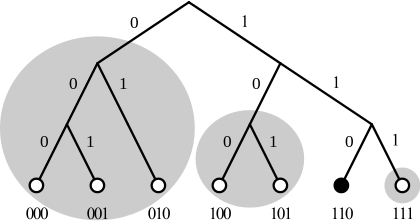
\includegraphics[width=.9\linewidth]{tree.png}
\captionof{figure}{Beispielhafte Darstellung eines einfachen Kademlia-Systems}
\end{center}

\noindent Mit dieser Sicht auf das System beschreibt die XOR-Funktion
die Anzahl der unterschiedlichen Abbiegungen im Baum und somit die
Distanz. Zwar mag es auf den ersten Blick nicht intuitiv wirken, wieso
man XOR anstatt einfach der Differenz verwendet, allerdings
funktioniert die Funktion mit Binärzahlen in einem solchen Baum
um einiges besser.
\item Routing-Table
\label{sec:orgecd335b}
In einem Kademlia-System hat jedes Mitglied eine gewisse Anzahl
anderer Mitglieder, mit denen es sich verbunden hat. Da Kademlia ein
sehr umfangreiches, kompliziertes Protokoll und System beschreibt,
sollen hier nur einige zentrale Funktionen besprochen werden, die für
diesen ersten Prototypen von Project Orion relevant sind.\\

\noindent Einfach formuliert speichert der \texttt{Routing Table} die
verbundenen Mitglieder. Eine eingehende Nachricht wird dann mithilfe
dieser Liste, sowie der XOR-Metrik ans richtige Ziel geschickt. Um das
System zu optimieren und die Anzahl der benötigten Sprünge klein zu
halten, wird ein spezielles System verwendet, um zu entscheiden,
welche Mitglieder im Routing-Table gespeichert werden sollen:

\begin{enumerate}
\item Sehr nahe an sich selbst (in der obigen Darstellung also:
wenige Sprünge im Baum) werden alle Mitglieder gespeichert.
\item Je weiter weg sich die Mitglieder befinden, desto weniger
werden gespeichert.
\end{enumerate}

\noindent Die optimale Anzahl der gespeicherten Mitglieder hängt von
den Zielen und Ansprüchen an das System ab. Grundlegend muss man die
Frage beantworten, mit wie vielen Unterbäumen Verbindungen gehalten
werden sollen. Zwar mag dies etwas abstrakt wirken, es lässt sich aber
mit dem eben eingeführten Modell eines umgekehrten Baumes gut
erklären:
\begin{itemize}
\item In der obersten Ebene trennt sich der Baum in zwei vollständig
getrennte Teile, was sich mit jeder weiteren Ebene wiederholt.
\item Die einzige Möglichkeit vom einen \emph{Ende} des Baums zum anderen
zu kommen, ist über den obersten Knoten. Um also in die andere
Hälfte zu kommen, braucht man mindestens eine Verbindungsstelle
in der anderen Hälfte.
\item Deshalb braucht ein Routing-Table nicht nur kurze
Verbindungen zu nahen Punkten, sondern auch einige wenige
Verbindungen zu Mitgliedern in der anderen Hälfte.
\item Mit nur einer weit entfernten Adresse hat man eine Verbindung
in die \emph{eigene} und die \emph{andere} Hälfte. Hat man zwei solche
Verbindungen auf die andere Seite hat man schon Verbindungen in
jeden Viertel des Baumes.
\item Man muss also entscheiden, wie fein man die andere Hälfte
aufteilen will. (Eine genaue Unterteilung bedeutet wenige
Sprünge aber grosse Routing-Tables, eine grobe Unterteilung
genau das Umgekehrte).
\end{itemize}

\noindent Zwar hat ein vollständiges Kademlia-System noch
komplexere Elemente, wie \texttt{k-Buckets}, welche den Routing-Table
optimieren, allerdings sind diese für die grundlegende
Funktionsweise des Systems irrelevant.\\

\noindent Die dynamische Regulation des Routing-Tables muss
allerdings noch erwähnt werden:
\begin{itemize}
\item Sobald die definierte Maximalgrösse erreicht ist, werden keine
neuen Verbindungen akzeptiert.
\item Zwar können existierende Einträge durch Neue ersetzt werden,
allerdings werden dabei nicht alte, sondern inaktive Einträge
entfernt. Für ein Kademlia-System werden also auch Mechanismen
benötigt, um die Zustände aller Verbindungen periodisch zu
überprüfen.
\end{itemize}
\end{enumerate}
\subsection{BitTorrent}
\label{sec:org5c7bb1a}
Dezentralisierung hat viele Vorteile und muss langfristig
flächendeckend eingesetzt werden. Aktuell sind die meisten
Industrien und Produkte noch nicht so weit. Trotzdem gibt es
einige Anwendungen und Gruppen bei denen solche Systeme bereits
seit Jahren Verwendung finden.\\

\noindent Beispielsweise im Zusammenhang mit der \emph{(mehr oder
weniger legalen)} Verbreiten von Materialien wie Filmen oder Musik
wird eines der grössten global verteilten Systeme eingesetzt.
Natürlich gibt es hunderte von verschiedenen Programmen, Ideen und
Umsetzungen, aber die meisten sind Nachfolger von \texttt{Napster}.\\

\noindent Im preisgekrönten Film \emph{The social network} erhält man
Einblick in den Lebensstil von Sean Parker, einem der Gründer von
Napster. Es mag überraschen, wie jemand wie Parker, der nur wenige
Jahre zuvor mit Napster die komplette Musikindustrie in Unruhe
gebracht hatte, eine so zentrale Rolle in Facebook, einem der
zentralisiertesten Megaunternehmen der Welt, einnehmen konnte.\\

\noindent Auch wenn es noch nicht \emph{vollständig} dezentralisiert ist,
erlaubte es Napster Nutzern, Musik über ein automatisiertes System
mit anderen Nutzern zu teilen und neue Titel direkt von den
Geräten anderer Nutzer herunterzuladen. Dabei gab es allerdings
immer noch einen zentralen Server, der die Titel sortierte und
indizierte. \\
Napster musste am Ende abgeschaltet werden, nachdem die Klagen der
Musikindustrie zu belastend wurden. Auch wenn das Produkt
abgeschaltet wurde, liess sich nichts mehr gegen die Idee
unternehmen.\\

\noindent Über viele Iterationen und Generationen hinweg wurden
die verteilten Systeme immer weiter verbessert, jegliche zentrale
Server entfernt und in die Hände immer mehr Nutzer gebracht. Heute
läuft ein Grossteil des Austauschs über \texttt{BitTorrent}.

\noindent BitTorrent baut auf der gleichen grundlegenden Idee wie
Napster auf: Nutzer stellen ihren eigenen Katalog an Medien zur
Verfügung und können Inhalte von allen anderen Mitgliedern im
System herunterladen. Anders als Napster gibt es bei BitTorrent
keine zentrale Komponente, stattdessen findet selbst das
Indizieren und Finden von Inhalten dezentralisiert statt\footnote{BitTorrent: Mainline DHT:
\url{https://www.cs.helsinki.fi/u/lxwang/publications/P2P2013\_13.pdf},
heruntergeladen am: 4.06.2020.}.
Dafür wird über das Kademlia-System aktiv bekannt gegeben, wer
welche Inhalte zur Verfügung stellt, wobei einzelne Mitglieder
speichern können, wer die gleichen Inhalte anbietet. Neben
Dezentralisierung und Sicherheit lassen sich über BitTorrent
tatsächlich gute Geschwindigkeiten erreichen, da sich Inhalte von
mehreren Anbietern gleichzeitig herunterladen lassen. Da es sich
bei BitTorrent eigentlich um ein grosses Dateisystem handelt,
lassen sich direkt die \texttt{SHA1}-Hashwerte der Inhalte als
Kademlia-Adressen verwenden.
\subsection{Tox}
\label{sec:orgf96c8e6}
Im Sommer 2013 veröffentlichte Edward Snowden schockierende
Geheimnisse über massive Spionage Prgogramme der NSA, mit welchen
nahezu aller digitaler Verkehr, ohne Rücksicht auf Datenschutz oder
Privatsphären mitgelesen, ausgewertet und gespeichert wurde. Nahezu
jede Person in der westlichen Welt war betroffen und das genaue
Ausmass ist bis heute noch schwer greiffbar. Vielen wurde aber klar,
dass sichere, verschlüsselte Kommunikation nicht mehr nur etwas für
Kriminelle und \emph{Nerds} war, sondern dass jeder Zugang zu
verschlüsselter, sicherer und dezentraler Kommunikation haben sollte.
In einem Thread auf 4chan wurden viele dieser Bedenken gesammellt und
es kam die Idee auf, selbst eine Alternative zu herkömmlichen Chat
Programmen wie Skype zu entwickeln. Aus dieser Initiative heraus
entstand Tox, wobei die Namen vieler der ursprünglichen Entwickler bis
heute unbekannt sind. Damals war das Ziel die Entwicklung einer
sicheren Alternative zu Skype, allerdings hat sich der Umfang des
Projekts inzwischen ausgeweitet. Im Zentrum der Arbeiten steht das Tox
Protocol, welches von verschiedenen, unabhängigen Programmen umgesetzt
wird. Zwar ist Chat weiterhin eine zentrale Funktion, es wird aber
auch mit Video- und Audiokommunikation sowie Filesharing gearbeitet.\\

\noindent Basierend auf der bekannten NaCl-Bibliothek\footnote{Crates.io: \url{https://crates.io/}} wird die
gesamte Kommunikation über das Tox Protocol\textsuperscript{\ref{orgc13932d}} zwingend end- zu
endverschlüsselt. Intern wird ein dezentrales Routing System,
basierend auf Kademila verwendet, mit welchem Kontakt zwischen Nutzern
(Freunden) aufgebaut wird. Während im Kademila Whitepaper Adressen mit
einer Länge von 20 Bytes definiert werden, nutzt Tox 32 Bytes. Dies
vereinfacht die Verschlüsselung stark, da NaCl Schlüssel verwendet,
welche ebenfalls 32 Bytes lang sind. Nebst der eingesparten
Verhandlung von Schlüsseln und der zusätzlichen Kommunikation bindet
diese Idee die Verschlüsselung stärker in das Routing System ein, denn
es werden keine zusätzlichen Informationen zum Verschlüsseln einer
Nachricht gebraucht, und sie kann direkt mit der Adresse des Ziels
verschlüsselt werden.\\

\noindent Es ist allerdings wichtig festzustellen, dass Tox Kademila
lediglich als Router verwendet. Kontakt zwischen zwei Nutzern wird
komplett dezentral hergestellt. Sobald diese sich allerdings gefunden
haben, wechseln sie zu einer direkten Kommunikation über UDP. Zwar
erlaubt diese Zweiteilung der Kommunikation schnellen Datenverkehr
sobald sich zwei Nutzer gefunden haben (so ist beispielsweise Video-
und Audiokommunikation möglich), es kommen aber auch einige neue
Probleme auf:
\begin{itemize}
\item Anders als beispielsweise im Darknet ist über das Onion-Routing von
Aussen klar erkennbar, mit wem jemand kommuniziert. Natürlich ist
der Inhalt weiterhin verschlüsselt, aber ein solches System setzt in
erster Linie auf Sicherheit und Geschwindigkeit und nicht auf
Anonymität.
\item Auch muss man bedenken, dass nicht jedes Gerät im Internet in der
Lage ist, direkte Verbindungen mit jedem anderen Gerät aufzubauen.
Besonders Firewalls können schnell zu Problemen führen.
\end{itemize}

\noindent Das Tox Protocol bietet eine einheitliche Spezifikation mit
der eine grosse Bandbreite an Problemen gelöst werden kann. Wer eine
sichere, dezentrale Alternative zu Whatsapp sucht, könnte an Tox
Gefallen finden. Seit einigen Jahren gibt es aber Bedenken über die
Sicherheit und aktuelle Richtung des Projekts, sowie Berichte von
internen Konflikten, besonders im Zusammenhang mit Spendengeldern.
\subsection{CJDNS}
\label{sec:org702f530}
Im CJDNS-Whitepaper werden viele der gleichen Probleme angesprochen,
wie auch hier erwähnt wurden. Die grundlegenden Ideen und
Lösungsansätze die besprochen werden ähneln in vielerlei Hinsicht den
Ideen und Prinzipien hinter Project Orion. CJDNS, das sich selbst als

\begin{center}
an encrypted IPv6 network using public-key cryptography for address
allocation and a distributed hash table for routing
\end{center}

\noindent beschreibt, ist ein beliebtes open-source Projekt, mit mehr
als 180 Mitentwicklern und tausenden von Nutzern. Es basiert ebenfalls
auf Kademlia und ähnlich wie BitTorrent wird grossen Wert auf
Sicherheit und Verschlüsselung gelegt.\\

\noindent Wer den Code von CJDNS etwas genauer anschaut realisiert
schnell, welche grundlegenderen Ziele CJDNS verfolgt. Tatsächlich soll
mit CJDNS langfristig ein physikalisch unabhängiges Netzwerk
entstehen. Das Whitepaper redet von der Freiheit der Nutzer, eigene
Kabel und eigene Infrastruktur zu verlegen.\\

\noindent Es mag auf manche nach digitaler Isolation und Abschottung
reden, aber wer tatsächlich konsequent alle Probleme von Grund auf
angehen will muss sich auch Gedanken über die darunterliegende
physikalische Infrastruktur machen. Dies ist allerdings ein Schritt
der mit Project Orion (noch) gemacht werden soll.
\section{Architektur}
\label{sec:orgfe0a6f5}
\subsection{Verschlüsselung}
\label{sec:orgda9be5a}
Zwar ist es bei weitem nicht so, dass alle moderne dezentrale Systeme
das Internet oder ein ähnliches Austauschsystem als Grundlage
verwenden, allerdings ist dies in nahezu allen Fällen, besonders bei
den beliebten und weit verbreiteten Fällen. Das Internet ist für
fehlende Sicherheit und Gefahren bekannt, daher ist es von Nöten, dass
sich jede Applikation selbst um Verschlüsselungen und Sicherheit
kümmert. Allerdings ist es wichtig, \emph{die passende Verschlüsselung} zu
wählen. Hier wird nun ein Ansatz beschrieben, welcher sich besonders
gut für gewisse Kademlia-inspirierte Systeme eignet. Dieser Ansatz
beruht auf der Verschlüsselungs-Bibliothek NaCl, beziehungsweise deren
modernen Abzweig \texttt{libsodium}. Während klassische
Verschlüsselungsmethoden sehr lange Schlüssel benötigen, gibt es
gewisse Kombinationen von Algorithmen, welche mit sehr kurzen
Schlüsseln Sicherheit gewährleisten können. Besonders geht es dabei um
curve25519xsalsa20poly1305, einer Kombination aus den Algorithmen
Curve25519, Salsa20 und Poly1305. Während das innere Zusammenspiel
dieser Algorithmen sehr komplex ist, ist das Resultat ein Algorithmus,
wessen Schlüssel jeweils nur eine Länge von \emph{32 bytes} haben.\\

\noindent Eigentlich beschreibt Kademlia Adressen mit einer Länge von
\emph{160 bits} (\emph{20 bytes}), allerdings ist es ohne grosse Probleme möglich,
die Adressen Länge auf \emph{32 bytes} zu verlängern. Dies erlaubt es uns,
die Verschlüsselung und das Adresssystem direkt miteinander zu
verbinden. Das mag auf den ersten Blick etwas umständlich und
unlogisch wirken, es erlaubt allerdings, ohne weitere Operationen,
verschlüsselte Nachrichten an einen Nutzer zu schicken, wobei
lediglich dessen Adresse bekannt sein muss. Insgesamt fällt damit viel
Komplexität weg und macht das Erstellen, Verifizieren und Finden von
Adressen viel einfacher.
\subsection{PubSub}
\label{sec:org1ec6c0a}
Ein einfaches, aber vielseitig einsetzbares
Nachrichtenübermittlungsmuster ist die Idee eines \texttt{Publish/Subscribe}
Systems. Ein solches System lässt sich mit nur zwei Aktionen
beschreiben: 
\begin{itemize}
\item Nutzer können ein gewisses Thema abonnieren, das bedeutet, sie folgen
einem gewissen Schlüssel und erhalten Nachrichten von diesem.
\item Jeder Nutzer kann dann in den Themen, die er abonniert hat
Nachrichten schicken. Diese werden dann automatisch an alle
abonnierten Nutzer verteilt.
\end{itemize}

\noindent Mit diesen beiden Mechaniken lassen sich die meisten
Funktionen in modernen Applikationen beschreiben. Sei es ein Chat-
oder Emailsystem, ein komplexer Datenverarbeitungsmechanisums oder ein
Datennetzwerk, alle lassen sich relativ einfach mit diesen beiden
Funktionen modellieren. 
\begin{enumerate}
\item Dezentraler PubSub
\label{sec:org18090d1}
Offensichtlich kann selbst die beste, fehlerfrei optimierte
Implementierung der oben beschriebenen Prinzipien nicht gegen die
bereits angesprochenen, fundamentalen Probleme lokal gebundener
Programme vorgehen. Daher ist es in einem nächsten Schritt von Nöten,
die Ideen hinter dezentralisierten \texttt{PubSub}-Systemen anzuschauen. Das
mag im ersten Moment komplex klingen, ist aber tatsächlich unglaublich
einfach. Man muss sich lediglich einen PubSub als zwei getrennte
Unterkomponenten vorstellen:
\begin{itemize}
\item Themen lassen sich vereinfacht als Einträge in einer Datenbank
beschreiben. Die Identifikation der Themen ist dabei der Schlüssel,
wobei die Abonnenten als dazugehörige Felder ausgedrückt werden
können. Oben wurde bereits ein System beschrieben, welches
zuverlässig dezentral Daten speichern kann. Wenn man in der
beschriebenen Kademlia Implementierung die Checksumme des Inhalts
mit der Checksumme des Themenschlüssels ersetzt, lässt sich Kademlia
ohne weitere Veränderungen für einen dezentralen PubSub einsetzen.
\item Danach bleibt natürlich noch das Problem der Nachrichtenverbreitung.
Dafür gibt es verschiedene Möglichkeiten:
\begin{itemize}
\item Die Nachrichten werden direkt an das zuständige Mitglied gesendet,
von dort werden sie weitergeleitet. Vorteilhaft an diesem Konzept
ist natürlich, dass die Verwender des Systems unglaublich einfach
gehalten werden können. Sie müssen lediglich Nachrichten an eine
Adresse schicken, das System kümmert sich dann von alleine um die
Weiterverbreitung. Damit geben die Nutzer allerdings auch eine
gewisse Kontrolle auf, denn sie können nicht direkt einsehen, an
wen ihre Nachrichten verteilt werden. In einer solchen Situation
gibt es zusätzlich noch gewisse technische Bedenken im
Zusammenhang mit der Verschlüsselung.
\item Andererseits dazu können auch die Aktionen des Abonnierens und
Deabonnierens als Nachrichten im System verbreitet werden. Jeder
abonnierte Nutzer wird somit also über neue Abonnenten informiert
und speichert deren Details lokal. Zwar erhöht dies die
Komplexität enorm, erlaubt aber schnellere Übertragung und genauer
Kontrolle über die Auswahl der Abonnenten.
\end{itemize}
\end{itemize}
\item Probleme
\label{sec:orge48ea8d}
Zwar gibt es viel Gutes über PubSubs als Systemkonzept zu sagen,
allerdings müssen auch einige Probleme angesprochen werden:
\begin{itemize}
\item Wie bereits eben angesprochen kann es zu gewissen Unklarheiten und
Problemen im Zusammenhang mit der Verschlüsselung der Nachrichten in
dezentralen Systemen kommen. Da Nachrichten meist über das offene
Internet übertragen werden und daher Verschlüsselung nahezu zwingend
benötigt wird, muss man sie auch hier berücksichtigen. Wie bereits
im Abschnitt zur Verschlüsselung angesprochen, sollen Nachrichten
mit dem öffentlichen Schlüssel des Empfängers, welcher auch
gleichzeitig die Adresse darstellt, verschlüsselt werden. Beim
Durchgehen der oben beschriebenen Architekturen wird ein Problem
offensichtlich: Wenn ein Thema ein normaler Empfänger im System ist,
muss seine öffentliche Adresse verwendet werden. Allerdings wurde
definiert, dass die Adresse eines Themas die Checksumme eines
bekannten Schlüssels darstellt. Die Adressen in einem solchen System
lassen sich allgemein aber durch einen gegebenen privaten Schlüssel
ableiten. Umgekehrt ist das natürlich nicht möglich. Ein geheimer
Schlüssel lässt sich nicht aus dem öffentlichen Schlüssel errechnen.
Hier wird also eigentlich ein System verlangt, bei welchem der
private Schlüssel durch eine Checksumme errechnet wird, wobei der
daraus entstehende öffentliche Schlüssel als Adresse verwendet wird.
Gleichzeitig darf der private Schlüssel nicht bekannt sein, sonst
wäre die gesamte Verschlüsselung sinnlos. Es wird schnell
offensichtlich, dass solche Bedingungen nie erfüllt werden können.
\item Da es sich bei der Liste der Abonnenten um Daten handelt, welche
während der Laufzeit gespeichert und verwaltet werden müssen, bringt
man plötzlich eine Vielzahl neuer Probleme ins Spiel. So müssen die
Daten repliziert und gesichert werden, da ein einzelnes Mitglied
jederzeit unerreichbar sein könnte. Sie müssen verifiziert werden,
da man kein Vertrauen in die Mitglieder des Systems haben darf und
sie müssen trotz häufiger Änderungen konstant gehalten werden. Das
Gebiet der dezentralen oder verteilten Datenbanken alleine ist sehr
gross und komplex, wenn man also plötzlich nebst einem
Nachrichtensystem ohne verteilte Zustände auch noch eine verteilte
Datenbank verwalten muss, übersteigt dies meist die erhoffte
Komplexität vieler Projekte.
\end{itemize}
\end{enumerate}

\section{Dokumentation}
\label{sec:orgb30e0d6}

\section{Glossar}
\label{sec:orgb9f9cf3}
In diesem Abschnitt sollen alle Begriffe, welche im Text mindestens
einmal \texttt{monospaced} geschrieben wurden, kurz erklärt werden.
\begin{itemize}
\item \texttt{Project Orion}: Maturaarbeit zum Thema \emph{Dezentrale Kommunikations- und
Datensysteme} von Dominik Keller und Jakob Klemm, Kanti-Baden, 2021.
\item \texttt{ARPANET}: Vorgängermodell des Internets, entwickelt vom
amerikanischen Verteidigungsministerium.
\item \texttt{FOMO}: Fear of missing out: Die Angst, Innovationen und Veränderungen
zu verpassen.
\item \texttt{IP-Adresse}: Eindeutige Identifizierung für Geräte im Internet.
Werden von Internetanbietern ausgestellt und sind meistens nur
eindeuting für einzelne Netzwerke, nicht Geräte, da diese ein
unabhängiges IP-Adress-System verwenden.
\item \texttt{TCP}: Transmission Control Protocol: Dominantes Protokoll um Daten im
Internet zu versenden. Grundlage für bekanntere Protokolle wie HTTP.
\item \texttt{UDP}: User Datagram Protocol: Simpleres und schnelleres Protokoll als
TCP, ist allerdings meist weniger zuverlässig.
\item \texttt{IP-V4}: Standardisierte Version der IP-Adressen mit einer Länge von
32 bit.
\item \texttt{IP-V6}: Neuste Version des Internet Protokolls mit einer Adresslänge
von 128 bit, allerdings inkompatibel mit IP-V4.
\item \texttt{POP-Switch}: Point of Presence: Von einem Internetanbieter
kontrollierter Knotenpunkt, der ein kleineres \emph{Subnet} abgrenzt.
\item \texttt{Zentralrouter}: Grössten und wichtigsten Knotenpunkte für den
globalen Internetverkehr, der grösste befindet sich in Frankfurt.
\item \texttt{Address Spaces}: Um Speicherplatz und Rechenleistung zu sparen,
werden komplette IP-Adressen an Firmen oder Gebiete vergebet.
\item \texttt{Shadow}: Orion Netzwerk-Router der ersten Entwicklungsphase,
geschrieben in Elixir.
\item \texttt{Elixir}: Programmiersprache für nebenläufige Programme, besonders
Netzwerke, basierend auf Erlang.
\item \texttt{Kademlia}: Peer to Peer Nachrichtensystem basierend auf der
XOR-Metrik.
\item \texttt{UNIX-Socket}: System zum Datenaustausch zwischen verschiedenen
laufenden Applikationen auf der selben Maschine.
\item \texttt{Hunter}: Lokaler Router der ersten Orion Entwicklungsphase.
\item \texttt{JSON}: Menschenlesbares Datei- und Nachrichtenstruktur für Objekte
und Schlüssel-Wert-Paare.
\item \texttt{Actaeon}: Dezentrales Nachrichtensystem der zweiten Orion
Entwicklungsphase.
\item \texttt{Rust}: Moderne Programmiersprache von Mozilla als Alternative zu C \&
C++.
\item \texttt{Crate}: Rust Terminologie für, von Nutzern entwickelte, Bibliotheken.
\item \texttt{XOR}: Logische Operation auf Binärdaten errechnet den Unterschied
zwischen zwei Eingaben.
\item \texttt{NaCl}: Verschlüsselungsbibliothek für Netzwerkprogramme.
\item \texttt{Interface}: Zentrale Zugangsstelle und Interaktionspunkt für die
Actaeon Applikation. Siehe Code Dokumentation für mehr Details.
\item \texttt{Topic}: Actaeon Datenstruktur die ein, im Netzwerk registriertes
Thema zu einem gewissen Schlüssel repräsentiert.
\item \texttt{CJDNS}: Initiative für ein technisch und physikalisch unabhängiges
Netzwerk als Alternative zum aktuellen Internet.
\item \texttt{Routing Table}: Gespeicherte Daten über bekannte Nodes in einem
Netzwerk zu denen Verbindungen aufgebaut werden können.
\item \texttt{k-Bucket}: Kademlia unterteilt den gesamten Routing Table in kleinere
Stücke, wobei alle Nodes in einem solchen Bucket in einen gewissen
Anteil ihrer Adresse übereinstimmen.
\item \texttt{Napster}: Eine der ersten Methoden illegal Musik direkt zwischen
Nutzern zu teilen.
\item \texttt{BitTorrent}: Aktuell beliebteste Methode um Medien und Daten aller
Art ohne jegliche Zentralisierung auszutauschen.
\item \texttt{SHA1}: Hash Algorithmus der einen Schlüssel mit einer Länge von 160
bit Produziert. Ursprünglich von der US-Regierung entwickelt.
\item \texttt{libsodium}: Moderne Umsetzung der NaCl Standards und Ideen.
\item \texttt{Publish/Subscribe} \& \texttt{PubSub}: Prinzip der indirekten
Nachrichtenübermittlung via Themen mit gemeinsamen Schlüsseln.
\end{itemize}

\includepdf[pages=-]{unterschrieben.pdf}
\end{document}
